\chapter{Theory}
\label{ch:Theory}

In this section we will discuss the theoretical background the project of this report is based on. As noted in \hyperref[sec:Objective]{the introduction}, the project aims at developing a proof-of-concept implementation of a Citizen Science accessible Liquid Democracy game. As such, it needs to be grounded in a thorough understanding of both the concept of \hyperref[sec:Theory_CS]{Citizen Science} and \hyperref[sec:Liquid_Democracy]{Liquid Democracy}. Additionally it needs to identify and address the problems and issues raised in relation to these concepts. 

In order to address these issues, a discussion of their context is indispensable. In recognition of this, the structure of this section is as follows:
After introducing the basic terms and the context they stem from (in \ref{ssec:Background_CS} and \ref{ssec:Liquid_Democracy}
respectively), issues and open questions are addressed for both concepts separately (in \ref{sec:Issues_CS} and \ref{ssec:LD-Critical-Perspective} respectively). 

Subsequently to a discussion on the background of the respective concept, we will \hyperref[sec:Integration_CSLD]{discuss synergies and challenges} of integrating these perspectives. Based on this integrative perspective and the aspects discussed at the beginning of this section, we will \hyperref[sec:Criteria]{derive a number of criteria} a Liquid Democracy game grounded in Citizen Science needs to exhibit, in order to develop a theory-grounded approach to the project's objective.

% Neu: Alternative

In this section, we will discuss the theoretical background the project is based on. As noted in the introduction, the project aims to develop a proof-of-concept implementation of a Citizen Science accessible Liquid Democracy game. As such, first of all, it is necessary to understand both the concept of Citizen Science and Liquid Democracy. Both terms are vast and used in many different backgrounds. Therefore, we will in the following section examine both terms separately, to then have a closer look on how the project itself combines Citizen Science and Liquid Democracy. In a first step, we will look closer at the term Citizen Science, it´s background and three theoretical perspectives on how to describe and classify a Citizien Science. Finally, we will summarize the common points of these three theories as well as open questions and difficulties a project of this nature might face.



% Clara
\section{Citizen Science}
\label{sec:Theory_CS}
\subsection{Background of Citizen Science}
\label{ssec:Background_CS}
Although Citizen Science in today’s academic world appears to be a rather contemporary term; the idea of Citizens being involved in the scientific process dates way back. Taking, for instance, the Christmas Bird Count. In 1900 the Ornithologist Frank Champman introduced the project involving volunteers in a yearly bird count on Christmas Day. Starting with 27 participants the number of volunteers over the years has been growing significantly. Until today scientists use the accumulated longitude data of around 53 000 active members for large scale analyses that have been crucial for findings around population, distribution of species and migration etc. With modern Technologies, the possibilities to involve Citizen in the scientific process have become more various which consequently has led to a rapidly growing amount of Citizen Science Projects. 

However, with increasing popularity, the term itself has become widely and rather differently used which makes it difficult to accurately define and differentiate it. Although the basic definition of involving members of the public in scientific research projects has remained this definition leaves several questions open: Which sort of participation and to which extent the citizens are involved in a project? What defines a citizen and what does it need to qualify a citizen science project? In the past several years researchers have tried to define more systematically what a citizen science means and what a CS project can consist of. In the following, we´ll look at two  different theoretical perspectives on Citizen Science Projects. 



\subsection{Types of Citizen Science Projects}
\label{ssec:Types_CS}
As mentioned before the number of Citizen Science Projects has expanded. Experience has shown that with thoughtful study design and under the right circumstances, citizen science can work on a massive scale, generating high-quality data that lead to reliable, valid scientific outcomes as well as unexpected insights and innovations. Therefore, more and more scientist involve Citizen Science project in their research process. Though looking at various CS Projects it quickly becomes  obvious that although they all involve some sort of citizen participation the projects themselves are quite different.  The researchers Andrea Wiggins and Kevin Crowston have therefore created a consisting typology, categorizing the projects into six different types. Examining common characteristics of 36 projects, grouping similar projects that share the same structure of participation, and some organizational as well as macro structural properties, Wiggis \& Crowston differentiate between Action-, Origination-, Conversation-, Investigation-, Virtual- and Educational Projects. Looking at the different kinds of projects they also summarize Scientific Organizational and Technology Issues common with this “mode” of Citizen Science. The following will briefly look at the different sorts of projects and summarize issues named: 

\subsubsection{Action Based Projects}
Action-oriented projects generally encourage participants to intervene in local concerns, using scientific research methods as a tool to support civic agendas. In contrast to other types of initiatives, an action orientated project materializes in form of a grassroots movement, as they are generally neither conceived nor planned by scientists. As an example, for an Action Project the text names the Sherman’s Creek Conservation Association, an organization with the goal to protect a local creek and to provide environmental education. In action-based projects, so Wiggis \& Crowston, researchers are often more consultants than collaborators. The, therefore, missing scientific method and spatial training generally prevent the collected data to become part of the scholarly knowledge base. The fact that these often are originated on a local level and is as well originated regarding local concerns cause the problem that there often lack funding and infrastructure which make it difficult for the project grow bigger than the original local level.

\subsubsection{Conversation Projects}
Conservation projects support stewardship and natural resource management goals, primarily in the area of ecology. Like Action projects, they are strongly rooted in local communes and volunteer engagement focuses on data collection activities, but in contrast to the Action projects, most conversation projects have affiliations with larger agencies.  Most projects include explicit educational goals or content. In regard to the scientific level, conversation projects often show a larger involvement of scientist and projects without strong academic affiliations are typically lead by professional researchers employed in governmental organizations. From an organizational point of view, it is interesting to observe that conversational oriented projects can be organized with top-down (researcher-initiated) as well as middle-out structures  (management-initiation). 

\subsubsection{Investigation Projects}
Investigation projects are in contrast to the conversational as well as the action based project focused on the scientific research goals which often consist of data collection. From this point of view, the Investigation Project fits the other definitions of Citizen Science Projects (Zitat .. Zitat) While education is not the foremost goal some material is often provided informing about the scientific background. Examples such as Great Sunflower and Fold Me (Galaxy Link) show that with this sort of project have to capacity to engage thousands of participants. Most Investigation projects involve or nonprofit conservation organizations as the primary organizers, and a top-down structure of organizing is a defining characteristic. Organizational Issues appear with a quickly growing number of participants as management and sustainability challenges grow accordingly.

\subsubsection{Education Projects}
As the name indicates the primary goal of education projects is education and outreach. An exemplary project here is Fossil Finders (Link). The project brings together educators, students as well as researchers developing workshops primarily for schools. Because of the created classroom atmosphere and supervised inquiry-based format, this particular project permits, on the one hand, a close involvement of the participants into the scientific process but on the other hand, it also facilitates the expansion and extension of the project activities, such as collection, identification, and description of additional fossils. Nevertheless, the emphasis on Education Projects lies in the educational aspect while scientific contribution is of secondary importance. Additionally, the relative cost of acquiring data through education projects is substantially higher. All the above often end in education projects only being considered as a Citizen Science project only by the virtue of including an academic institution or researcher as an organizer. Proceeding to the organizational issues, it is hardly surprising that all of  Wiggis \& Crowston´s sample projects are top-down organized. Involving multiple partners the examined project all have substantial funding.

\subsubsection{Virtual Projects}
In contrast to all other project types described above, Virtual Projects are completely ICT-mediated with no physical element whatsoever. The exclusively virtual based project shares its´ goal with the Investigation project as its´ main focus is the scientific research often in form of data collection. While examples of these projects are numerous, Galaxy Zoo, Whale FM and Planet hunter, just to name view, the line to projects that not further fall under the definition to Citizen Science is narrow. Depending on if Citizen Science here is defined as Citizen Participation in the project or includes in active involvement in to research project, Virtual projects often run danger to not match the definition of a citizen science project. The researcher Hackley looks closer at this problematic in his article .... In paragraph ...  we will further discuss this differation and Hackley ´s vision of the topic. Focusing on the Scientific Issues. As for Investigation projects, the primary challenge for Virtual projects is ensuring valid scientific results. This matter is complicated by the fact that is rather difficult to maintain the volunteer's´ interest. Even though motivation concerns are often addressed by game-like task design, it is often difficult to collect valid data. Many virtual projects compensate the missing quality of the data with task repletion. Nevertheless, this problematic is worth keeping in mind. Looking at the organization of Virtual projects, Wiggis \& Crowston conclude that all of their examined projects are top-down organized and exclusively run by academics. Consequently, the projects are most and foremost financed by research funding and interest what often poses a threat to the project´s sustainability.

\subsection{Haklay´s Ladder of Participation}
\label{ssec:Ladder_Participation_CS}

As already noted the extent to which volunteers are involved in a Citizen Science Project plays a crucial part regarding the nature of the project. To qualify as a Citizen Science Project the non-professional scientist must play some sort of active role in the research process.  This “ active” role however can be a lot, form discovering objects in pictures like in the mentioned Galaxy Zoo project to finding, describing and identification of actual Fossils. To closer define this rather large spectrum of participation the researcher Muki Haklay introduces the \textbf{Ladder of Participation} distinguishing between 4 different levels of involvement. At the most basic level, participation is limited to the provision of data/resources and minimal cognitive engagement. Hacklay titles this level of participation \textbf{Crowdsourcing} as volunteers often barely function as better sensors. 

The next level is the so-called \textbf{Distributed Intelligence}. Here the cognitive ability of the participants is crucial. Many Citizen Science Projects operate on this level. Volunteers are needed to take some basic training to collect data or carry out simple interpretation activity. On this level of engagement volunteers with time can learn more about the topic and advance beyond their initial training and be given more advanced tasks.

What distinguish the next level \textbf{Participatory Science} is that the volunteers are involved not only in the data collection but in the problem definition. As shown in the above mentioned  Fossil Finder Project the participants are on the one hand engaged in the data collection but with the assistance of experts are also taking part in the analysis and interpretation of the results.  Participants can suggest research question, which than can be explored with the data collected. 

The last and highest level on the ladder is the level of \textbf{Collaborative Science}. Here the participants can choose their level of engagement and can be potentially involved in analysis publication or utilization of the results. In addition to their role as experts, scientists here function as facilitators. This mode of Citizen Science, so Hacklay, even opens the possibility of citizen science without professional scientists.

Summarizing Hacklay states, that one project not necessarily have to be classified in only one category. Seeing for example the volunteer computing projects. While most participants will start  at the bottom level, collecting data or carrying out basic interpretation, some volunteers  might move to the second level assisting or teaching other volunteers. According to Hacklay some participants might even move one lever up and communicate with the scientists discussing results or suggest new research directions. It can be concluded that participation in Citizen Science can take different forms, while in some projects the gap between professional scientist and participants is wide, some other facilitate collaboration, teaching volunteers so they can become more involved in the scientific process altogether.

\newpage

\subsection{Issues and Open Questions}
\label{sec:Issues_CS}

Both Wiggis \& Crowston and Hackley agree, that the number, as well as the diversity of Citizen Science Projects, are vast. Nevertheless, the objective to include citizens in the scientific process itself sometimes seems to be at the very core of the project and other times more of a side effect. It also appears that even though the number of Citizen Science projects is growing, the data sill is used cautiously in papers and scientific publications. (Hackley) This seems especially the case for projects in which the influence of scientist is relatively small. The authors Flanagin and Metzger state that this might be originated in the fact that many researchers still mistrust the quality of the data produced by citizens. While Holling ( 1998 ) emphasized that there are two cultures of science and that citizen science by necessity belongs to the type of science that incorporates uncertainty and highlights integrative approaches.

Another question left open is what exactly defines a Citizen and what a Scientist. Through the preceding text, we deliberately have left this question open as Citizen Science itself to some extent questions the classic definition Science itself. Defining a scientist as someone being employed to carry out scientific work or research the differentiation stays rather clear. But as soon as it comes to unpaid scientists the situation is far more complex. It would mean to define scientists throughout their way of working with scientific frameworks, data collection, and interpretation as well as their overview and knowledge about the field, being able to place the newly won information in the already existing body of work. Nevertheless, pursuing this definition a well-trained and informed Citizen could then also meet these criteria. Authors like Irwin ( 1995 ), Wilson et al. ( 2005 ) and Stilgoe ( 2009 ) take this thought process one step further declaring that changing the epistemology of science could be seen as one goal of Citizen Science. They advocate that on a “extreme” level of Citizen Science the emphasis shouldn´t be on the citizen as a scientist but the scientist as a citizen. Meaning that in some cases it shouldn´t be possible to draw the line between Scientist and Citizen. However, Irwin ( 1995 ) also notes that this way of conceptualizing and practicing science is not widely accepted in the current culture of science.


\section{Liquid Democracy}
\label{sec:Liquid_Democracy}

Even though there are many forms of political government, it is democracy that spread around the globe over the last hundred years (see \autoref{fig:democracy-trend}). \textit{“As of the end of 2016, 97 out of 167 countries (58\,\%) [\ldots] were democracies [\ldots]”} \parencite{Desilver2017}. According to the observations in \autoref{fig:democracy-trend} it can be argued that democracy is a successful and thus modern structure, since there is no competing political system showing a similar thriving trend as democracy does.

\begin{figure}[H]

	\centering \begin{tikzpicture}
	\node[anchor=south west,inner sep=0] (image) at (0,0,0) {\includegraphics[width=8cm]{democracy-trend.png}};
	\begin{scope}[x={(image.south east)},y={(image.north west)}]
% 	% next four lines will help you to locate the point needed by forming a grid. comment these four lines in the final picture.↓
% 		\draw[help lines,xstep=.1,ystep=.1] (0,0) grid (1,1);
% 		\draw[help lines,xstep=.05,ystep=.05] (0,0) grid (1,1);
% 		\foreach \x in {0,1,...,9} { \node [anchor=north] at (\x/10,0) {0.\x}; }
% 		\foreach \y in {0,1,...,9} { \node [anchor=east] at (0,\y/10) {0.\y};}
% 	% upto here↑
    
	\libertineLF
	\draw (-0.05,0.0) node {\small{0\,\%}};
    \draw (-0.06,0.2) node {\small{20\,\%}};
    \draw (-0.06,0.4) node {\small{40\,\%}};
    \draw (-0.06,0.6) node {\small{60\,\%}};
    \draw (-0.06,0.8) node {\small{80\,\%}};
    \draw (-0.07,1.0) node {\small{100\,\%}};
   	\libertineOsF
    \draw (0.0,-0.06) node {1816};
    \draw (0.17,-0.06) node {1850};
    \draw (0.425,-0.06) node {1900};
    \draw (0.67,-0.06) node {1950};
    \draw (0.93,-0.06) node {2000};
    
	\draw[-latex] (0.99,0.25) -- +(0.5cm,0cm)node[anchor=west] {\scriptsize{Democracy}};
    \draw[-latex] (0.99,0.6) -- +(0.5cm,0cm)node[anchor=west] {\scriptsize{Open Anocracy}};
    \draw[-latex] (0.99,0.695) -- +(0.5cm,0cm)node[anchor=west] {\scriptsize{Closed Anocracy}};
    \draw[-latex] (0.99,0.85) -- +(0.5cm,0cm)node[anchor=west] {\scriptsize{Autocracy}};
    \draw[-latex] (0.99,0.96) -- +(0.5cm,-0.28cm)node[anchor=west] {\scriptsize{Colony}};
    \draw[-latex] (0.99,0.98) -- +(0.5cm,0cm)node[anchor=west] {\scriptsize{Transition/No data}};

	
	\end{scope}
	\end{tikzpicture}
	\caption[World population by political regime]{World population by political regime \parencite[see][]{Roser2018}.}
	\label{fig:democracy-trend}

\end{figure}
Nevertheless, it is neither within the scope of this project to asses democratic characteristics, nor other systems of rule. Democracy, however, entails various advantages compared to other political systems. First and foremost---by its literal translation\footnote{\textit{Rule of the people}, from Ancient Greek: \textgreek{Δημοκρατία} (Dēmokratía): democracy, whereby \textgreek{Δῆμος} (Dêmos) means \textit{the people}, and \textgreek{Κράτος} (Krátos) means \textit{power/strength}.}---democracy empowers its citizens to participate in political processes, and therefore to influence the political pathway. For example, one fundamental element is suffrage, that is, the right to vote. Additionally, democracy allows its people to shape the system’s frame. Thus, a wide range of democracy types\footnote{For further reading see the Wikipedia article \textit{Types of democracy}: \url{https://en.wikipedia.org/wiki/Types_of_democracy}.} have evolved over time. In this project we focus on \textit{liquid democracy}, a variant of democracy that is also known as \textit{delegative democracy}.


\subsection{Liquid Democracy Terminology}
\label{ssec:Liquid_Democracy}

Liquid Democracy (\tracknshrink{LD}) is a type of democracy lying in between two major democracy forms: direct democracy and indirect (or representative) democracy. This \textit{liquid} intersection allows citizens to either delegate their vote to a proxy (i.e., a representative) or to vote directly for a certain state of affairs (e.g., a proposition).

It is important to point out that the voting form \textit{proxy voting} shares some similarities of liquid democracy. There is, however, a fundamental difference: in liquid democracy a proxy may further delegate his/her voices to another proxy, which is not intended for proxy voting. Therefore, a proxy or representative, in the concept of liquid democracy, can be---mathematically---interpreted as a transitive (recursive) vertex within a directed graph. \citeauthor{Kahng2018} states:

\begin{displayquote}
“In contrast to the classic proxy voting paradigm \parencite{Miller1969}, the key innovation underlying liquid democracy is that proxies [\textellipsis] may delegate their own vote to a proxy, and, in doing so, further delegate all the votes entrusted to them. Put another way [\textellipsis] votes may freely flow through the directed delegation graph until they reach a sink.”\\[1mm]
\hspace*{\fill}\textcite{Kahng2018}
\end{displayquote}
The delegation graph is a fundamental component of liquid democracy. \autoref{fig:Delegation-Cascade} visualizes such a delegation graph/cascade. 

\begin{figure}[H]
\centering
\includegraphics{delegation-cascade.png}
	\caption[Delegate cascade voting]{“A snapshot of a small election in which two separate cascades have formed. Vote flow is depicted by arrows, and volume by numbers. The votes flow together until they pool at the bottom, where they are held by the leading candidates.” \parencite{Allen2008}}
	\label{fig:Delegation-Cascade}
\end{figure}
However, direct voting is neither intended in proxy voting nor in delegation graphs. Therefore---and to fulfill the initial definition of \tracknshrink{LD}---the delegation graph must be extended to permit direct voting, which then allows to further classify the terms: proxy voting, delegation graph and liquid democracy in a true subset relationship: \textit{proxy voting \(\subsetneq\) delegation graph \(\subsetneq\) liquid democracy}. Thus, the concept of liquid democracy acts as a superset for proxy voting and delegation graphs. 

\subsection{Liquid Democracy Mechanics}
\label{ssec:Liquid_Democracy_Mechanics}

Due to its superset position liquid democracy combines characteristics from proxy voting, delegation graphs and direct voting. To visualize this concept in a simplified manner \autoref{fig:Liquid-Democracy-Delegated-Voting} illustrates the main steps of a voting process within a liquid democracy system.

In liquid democracy, and in directed delegation graphs, the vote always flows from a \textit{principal}\todo{explain Proxy with a reference} to a \textit{proxy}, and, initially, each citizen always starts as a  principal holding their own voice, as depicted in the first column in \autoref{fig:Liquid-Democracy-Delegated-Voting}. From there, each individual has two choices: (1) to vote \textit{directly} for a given state of affairs (Option A, B or C) or (2) to \textit{delegate} their voice to a 
proxy. Naturally, and for the sake of completeness, citizens have the right to abstain from voting at all, however, in this work we set the focus on people seeking for participation. Thus, choice (1) entitles citizens to \textit{directly} influence a given state of affairs, as depicted in red. Apparently, voting as a ‘initial principal’ yields to the lowest voting impact of \(1\), which is by definition your own inherent voice. Choice (2) entitles citizens to \textit{delegate} their voice to a proxy, which can be the case when the (initial) principal is doubtful in their decision-making (\textit{uncertainty} is depicted by gray color in \autoref{fig:Liquid-Democracy-Delegated-Voting}).

If, however, an individual receives a single voice or multiple voices they automatically become a proxy. In this position they have the same two choices as the principals had before, that is, to either directly vote or to further delegate their votes. This characteristic demonstrates the recursive nature of a liquid democracy system. In the case of an uncertain proxy (column two, \autoref{fig:Liquid-Democracy-Delegated-Voting}), the proxy might further delegate their voices. Technically, by doing so, the proxy becomes a principal, yet with a higher voting impact, since the voting count gets accumulated along the graph, whereby each node has a natural weight of \(1\).

Ultimately, each edge will hit at some point their last node, which are---in a liquid democracy system---individuals being certain about their decision-making and have an opinion (\textit{certainty} is depicted by colors in \autoref{fig:Liquid-Democracy-Delegated-Voting}). In this step there are no further delegations.

\begin{figure}[H]
	\centering \begin{tikzpicture}
	\node[anchor=south west,inner sep=0] (image) at (0,0,0) {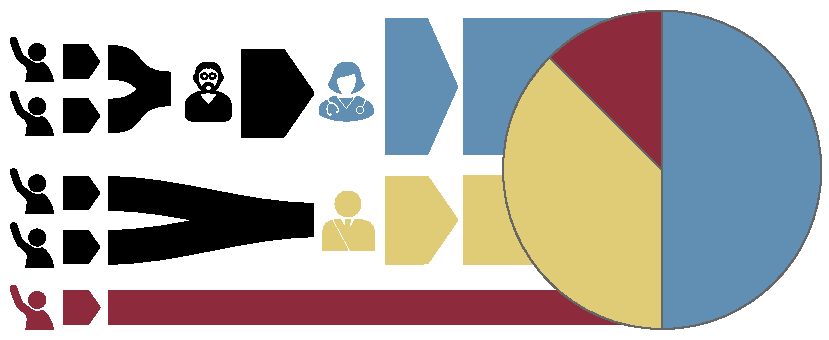
\includegraphics[width=\linewidth]{Liquid-Democracy-Delegated-Voting.pdf}};
	\begin{scope}[x={(image.south east)},y={(image.north west)}]
% 	% next four lines will help you to locate the point needed by forming a grid. comment these four lines in the final picture.↓
% 		\draw[help lines,xstep=.1,ystep=.1] (0,0) grid (1,1);
% 		\draw[help lines,xstep=.05,ystep=.05] (0,0) grid (1,1);
% 		\foreach \x in {0,1,...,9} { \node [anchor=north] at (\x/10,0) {0.\x}; }
% 		\foreach \y in {0,1,...,9} { \node [anchor=east] at (0,\y/10) {0.\y};}
% 	% upto here↑
    
    \draw (0.045,1.03) node {\textsf{\textbf{Principal}}};
    \draw (0.250,1.03) node {\textsf{\textbf{Proxy 1}}};
    \draw (0.415,1.03) node {\textsf{\textbf{Proxy n}}};
    \draw (0.580,1.03) node {\textsf{\textbf{Option}}};
    \draw (0.800,1.03) node {\textsf{\textbf{Results}}};
    
    \draw[line width=0.1mm] (0,0.992) -- (0.98,0.992);
    
    \draw (0.068,0.730) node {\textcolor{gray}{\(\textsf{\footnotesize{1}}\)}};
    \draw (0.068,0.571) node {\textcolor{gray}{\(\textsf{\footnotesize{1}}\)}};
    \draw (0.068,0.353) node {\textcolor{gray}{\(\textsf{\footnotesize{1}}\)}};
    \draw (0.068,0.193) node {\textcolor{gray}{\(\textsf{\footnotesize{1}}\)}};
    \draw (0.068,0.002) node {\textcolor{gray}{\(\textsf{\footnotesize{1}}\)}};
    
    \draw (0.280,0.618) node {\textcolor{gray}{\(\textsf{\footnotesize{3}}\)}};
    \draw (0.450,0.618) node {\textcolor{gray}{\(\textsf{\footnotesize{4}}\)}};
    \draw (0.450,0.232) node {\textcolor{gray}{\(\textsf{\footnotesize{3}}\)}};
    
    \draw (0.58,0.74) node {\textsf{\textcolor{white}{\textbf{A}}}};
    \draw (0.58,0.35) node {\textsf{\textcolor{white}{\textbf{B}}}};
    \draw (0.58,0.10) node {\textsf{\textcolor{white}{\textbf{C}}}};
	
	\end{scope}
	\end{tikzpicture}
    \caption[Illustration of liquid democracy]{Illustration of a liquid democracy system. Each individual has a voice, depicted by the numbers. Citizens may either vote directly or delegate their voice. Delegation will accumulate the voice impact for a proxy. Certainty is color-coded, whereas uncertainty is gray-coded.\\
    \hspace*{\fill}
    \scriptsize{\textit{Icons provided by thenounproject.com under Creative Commons 
\includegraphics[height=\fontcharht\font`\X]{cc-icon.pdf} license}}\\
    \hspace*{\fill}
    \tiny{\textit{
    	\url{https://thenounproject.com/icon/575955/}, 
    	\url{https://thenounproject.com/icon/24402/},\\
    	\hspace*{\fill}
        \url{https://thenounproject.com/icon/751412/}, 				\url{https://thenounproject.com/icon/1471169/}
        }}
	\label{fig:Liquid-Democracy-Delegated-Voting}}
\end{figure}

\subsection{Critical Perspective}
\label{ssec:LD-Critical-Perspective}

Allen nach oben und den Abuse hier rein

There is a variety of scientific articles and questions that are widely discussed in various online platforms (see REFERENCES). For this report we highlight some of them in regards
we assume that voters can only delegate their votes to better-informed voters \parencite{Allen2008}


Traditionally, in a parliamentarian democracy, the right to initiate and vote on propositions is exclusive for members of the parliament.
However, in a liquid democracy, by definition every participant has the right to vote on propositions, and participate in their constitutive phase.
Consequently, every participant should also have the unrestrained right to create propositions.

\subsection{Digital Liquid Democracy}

\label{ssec:Issues_LD}
\section[An Integrative Perspective for CS in LD]{An Integrative Perspective for Citizen Science in Liquid Democracy}
\label{sec:Integration_CSLD}

\todo[]{Hier muss eine Verbindung von Citizen Science und Liquid Democracy und zu unserem Projekt rein.}

\subsection{Data Accessibility and Anonymity}
\label{ssec:Integration_AccessibilityAnonymity}
Arguably the most challenging aspect of a CS-based LD platform, is the tension between data accessibility and anonymity. As stressed \todo{actually stress it!} in \ref{ssec:Issues_LD}, vote anonymity is a crucial aspect of democratic voting systems. On the other hand, a lack of transparency and data accessibility \todo[inline]{reduces the Citizen Scientist} to a data provider, devoiding a system of its participatory nature and transforming it into a mere crowd-sourcing platform (from a CS perspective). In order to allowing Citizens to pose (and investigate) research questions based on real-world data within their context of interest and expertise, as well as for delegators to evaluate whether their values are represented appropriately by delegants, data accessibility / transparency (at least to some degree) is imperative.

Although at first glance transparency and anonymity might seems like a null-sum-game where increased data accessibility constitute a violation of a users privacy, a number of strategies do exists that tackle these problems.

\subsubsection{Decoupling User Accounts from Personal Identity}

The most obvious strategy might be to decouple the user account from the personal identity of a user. When done consecuently, with proper protection of data (and the personal identity of the user is used solely to validate the vote connected to the account, or even just the existence of the account), all data of the user can be transparent by everyone, and no restrictions on the data accessiblity needs to be enforced. While this is the optimal solution from the perspective of the Citizen Scientist, and the delegator that can (in theory) perfectly evaluate whether her political power was used as intended, this approach is not without danger.

First, and most obviously, this approach is very problematic when a breach of the separation of the user and personal identity of the user occurs. Perfect safety does not exist, and many cases where sensitive (and this would be highly sensitive) information was exposed do exist (citation needed). More subtly however, with perfect accessibility of user data, with more and more detailed data, increasingly detailed profiles can be constructed, which are more and more likely to be bound to a person by tying their democratic persona to their personal identity (citation needed). While this might be somewhat harder for 'non-public' persons, for people active in the public sphere by their personal identities (e.g. politicians), this link would be easy to establish. One thoughtless given detail might be enough to link the entirety of the user persona to the human behind their account, making transparent in its entirety all activity and views every uttered on the platform. 

Most problematic about this issue from a participatory democratic perspective is the mechanics that more involvement leads to a higher probability of (someone sufficiently clever) the user persona being linked to the person behind this, thus rather discouraging than encouraging engagement in the participatory processes.

\subsubsection{Aggregating User Data}

Another, rather conservative solution for this issue would be to anonymize the user data by aggregating voting behaviour by demographic aspects of users. A scientist would thus get access to the distribution of voting patterns, vote delegation patterns or involvement in issues by certain demographics. Though preserving the anonymity and privacy integrity of the person behind a user, it has two shortcomings. First, this employs a conservative empiric perspective (since science by demography is out and attitude and behaviour, as well as cognitive patterns are en vogue (citation needed)). Second, this enables the interested scientist only to ask one type of question. The form of the research question is thus already pre-determined by the designers of the platform, and the demographic categories users provide. While this doesn't hinder Citizen Scientists to design and perform studies on the data, this doesn't realize the high participatory level of involvement in the research process that we would strive for in this project.

An aspect not addressed by this perspective is how much information a delegator would receive about the delegant (and the delegants it re-delegates the vote to). Since the usage of the single vote of the delegant is of interest, an aggregated perspective does not answer how well he could ensure his values are respected. With absolute transparency of the behaviour of the delegant to the delegator, a malign and smart (group of) delegators could derive information that would validate this paradigm.

\subsubsection{Deflecting Responsibility}

An easy, yet cowardish, third option for dealing with this problem would be to shift the responsibility for this from the platform's designers or operators to the users. Users could decide how much information they want to make available to other users / scientists and their delegators. While this has the chance to solve the problem and pay users the respect of being mature enough to decide this, this might lead to transparency pressure that every user that wants to accumulate political power needs to justify himself. Maybe deciding to pay this price is what can be expected from a politician, but this decision should not be engrained in the architecture of the platform. How easy such a setup would be for a scientist who has to deal with (potentially a lot of) partial information needs to be evaluated.

\subsubsection{Selective Aggregation}

A further, much more involved option would be to 'hide' unaggregated information for inquiring scientists, and to allow only information of a certain level of aggregation. Though similar to the second option posed above, this is quite a different approach to the problem at hand, since this approach explicitly opposes restricting research questions to a set / style of pre-formed research questions. The idea behind this approach is to allow all \textit{kind} of data inquiries, as long as certain criteria are met. These criteria are thought to ensure the anonymity of the user identity against inquiring entities, and would be the main design issue of this concept. As an example, criteria could be quantitative, only allowing access to data with a given amount of entities. This could be realized e.g. through a data query language with a filter instance, only allowing responses on data instances of a given size (in the style of 'how many people that voted like this in elections of this context voted like that / delegated votes' with a negative response when there are only a handful of instances and a valid answer when there are a substantial number of instances). Establishing these criteria would probably result in a lot of (hard) work, but might well be worth it. Whether research would be possible with the partial answers this approach generates, is a different question altogether. 
This approach further doesn't give an answer to transparency of vote delegation for individual political subjects raised above.

%\subsection{Theorien aus Liquid Feedback}
\section{Criteria for a CS based LD Platform}
\label{sec:Criteria}

In an anonymized large-scale digital liquid democracy, this right could be abused by malicious users to mass-create so called spam propositions in order to bury other propositions and prevent users from voting on them.
We aim to reduce this threat through the following measures: (1) phased proposition life cycles, (2) adaptive sorting algorithms based on bayesian filtering and (3) moderation.